\documentclass{article}
\usepackage[utf8]{inputenc}

\title{PS6}
\author{Travis Richardson }
\date{March 2019}

\usepackage{natbib}
\usepackage{graphicx}

\begin{document}

\maketitle

\section{Cleaning the Data}
I was not sure how to clean the data and add the steps on R. For this, I cleaned the data in the Excel sheet that I had and uploaded the edited version into R. However, the steps I took to clean and transform the data were: 1. Put the teams in alphabetical order and list amount of wins and goals they had within the last 12 seasons. 2. I gathered all of Arsenal's information for the last 12 seasons and put them separated from other teams. 3. Added the final league position for each year next to both Arsenal. Step 1, helps with a graph to look at goals compared to wins for every team that has participated in the EPL for the last 12 years. Step 2 is to look at Arsenal individually. And step 4 was to further the comparison between Arsenal. 
\section{Wins Compared to Goals}
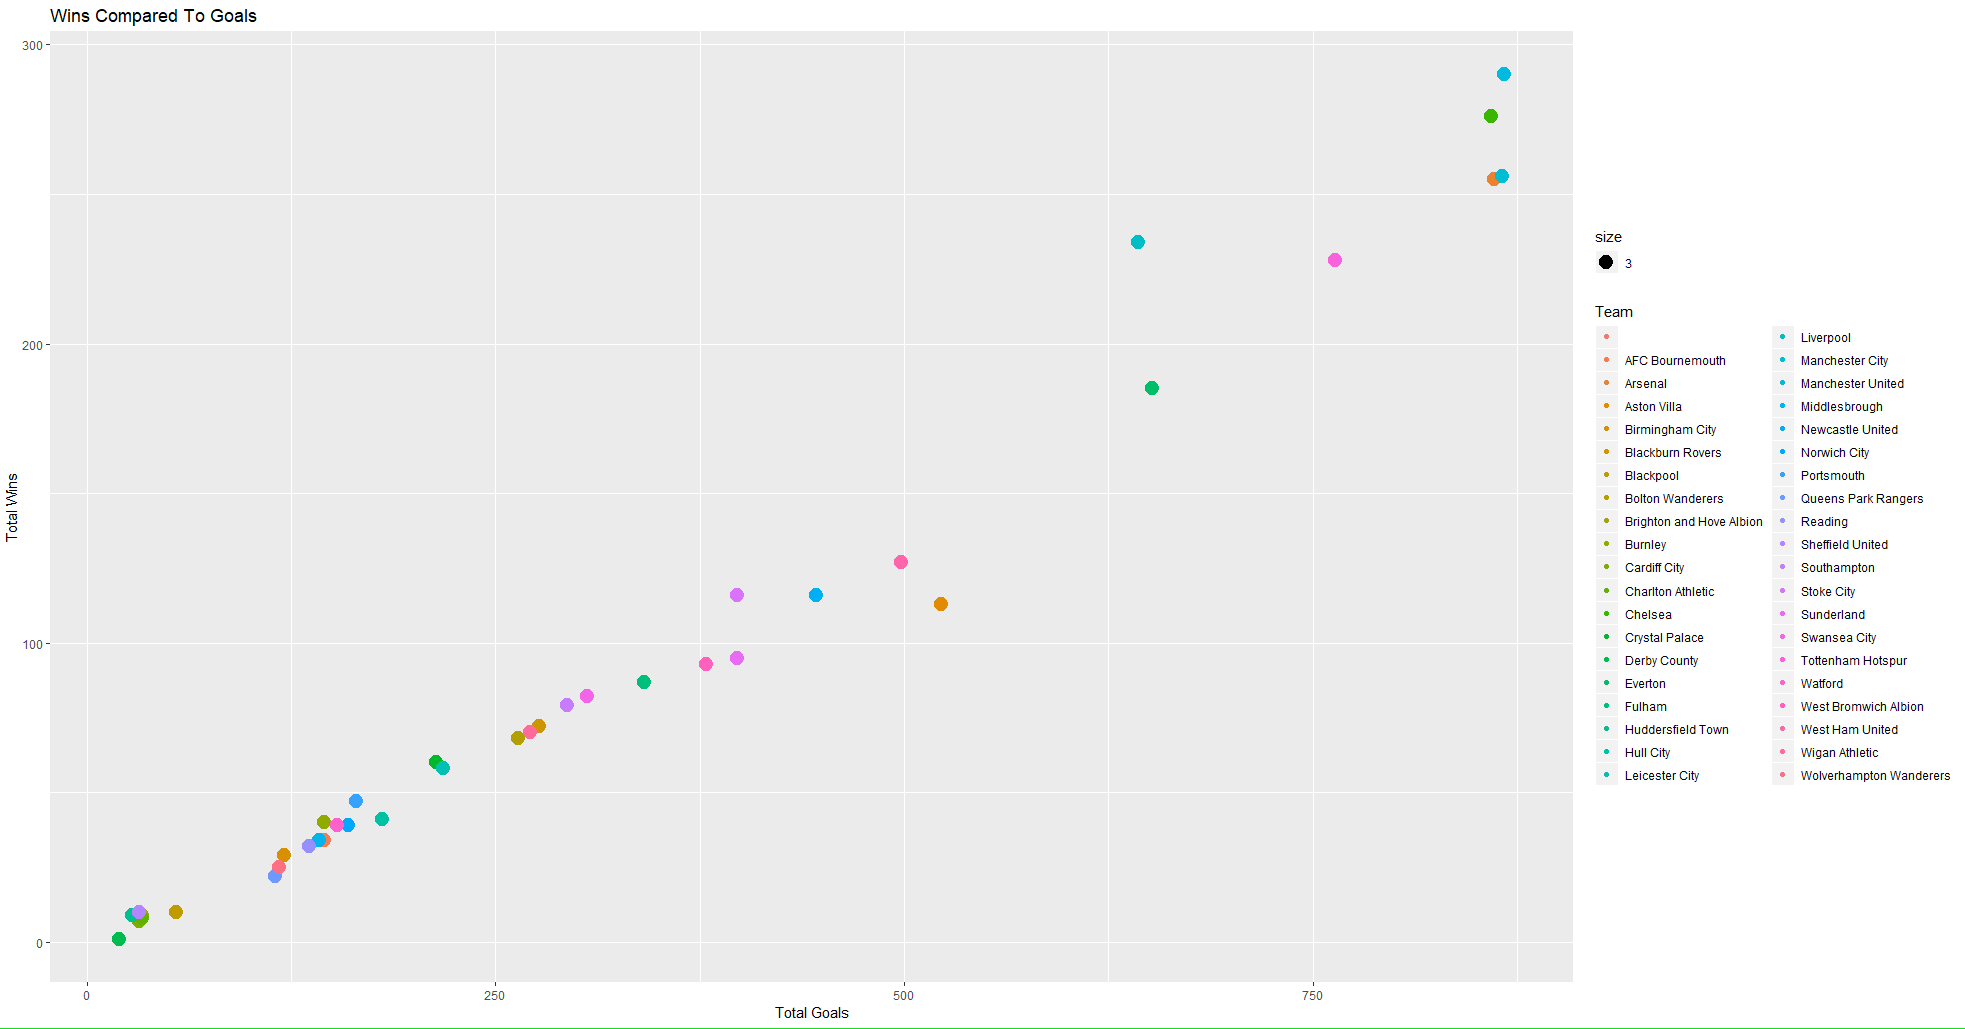
\includegraphics[width=\textwidth]{PS6a_Richardson}
This first graphic represent every team that participated in the EPL over the past 12 years, whether it be for one season or all twelve seasons, and how many wins they had compared to goals scored.
\section{Wins per Season}
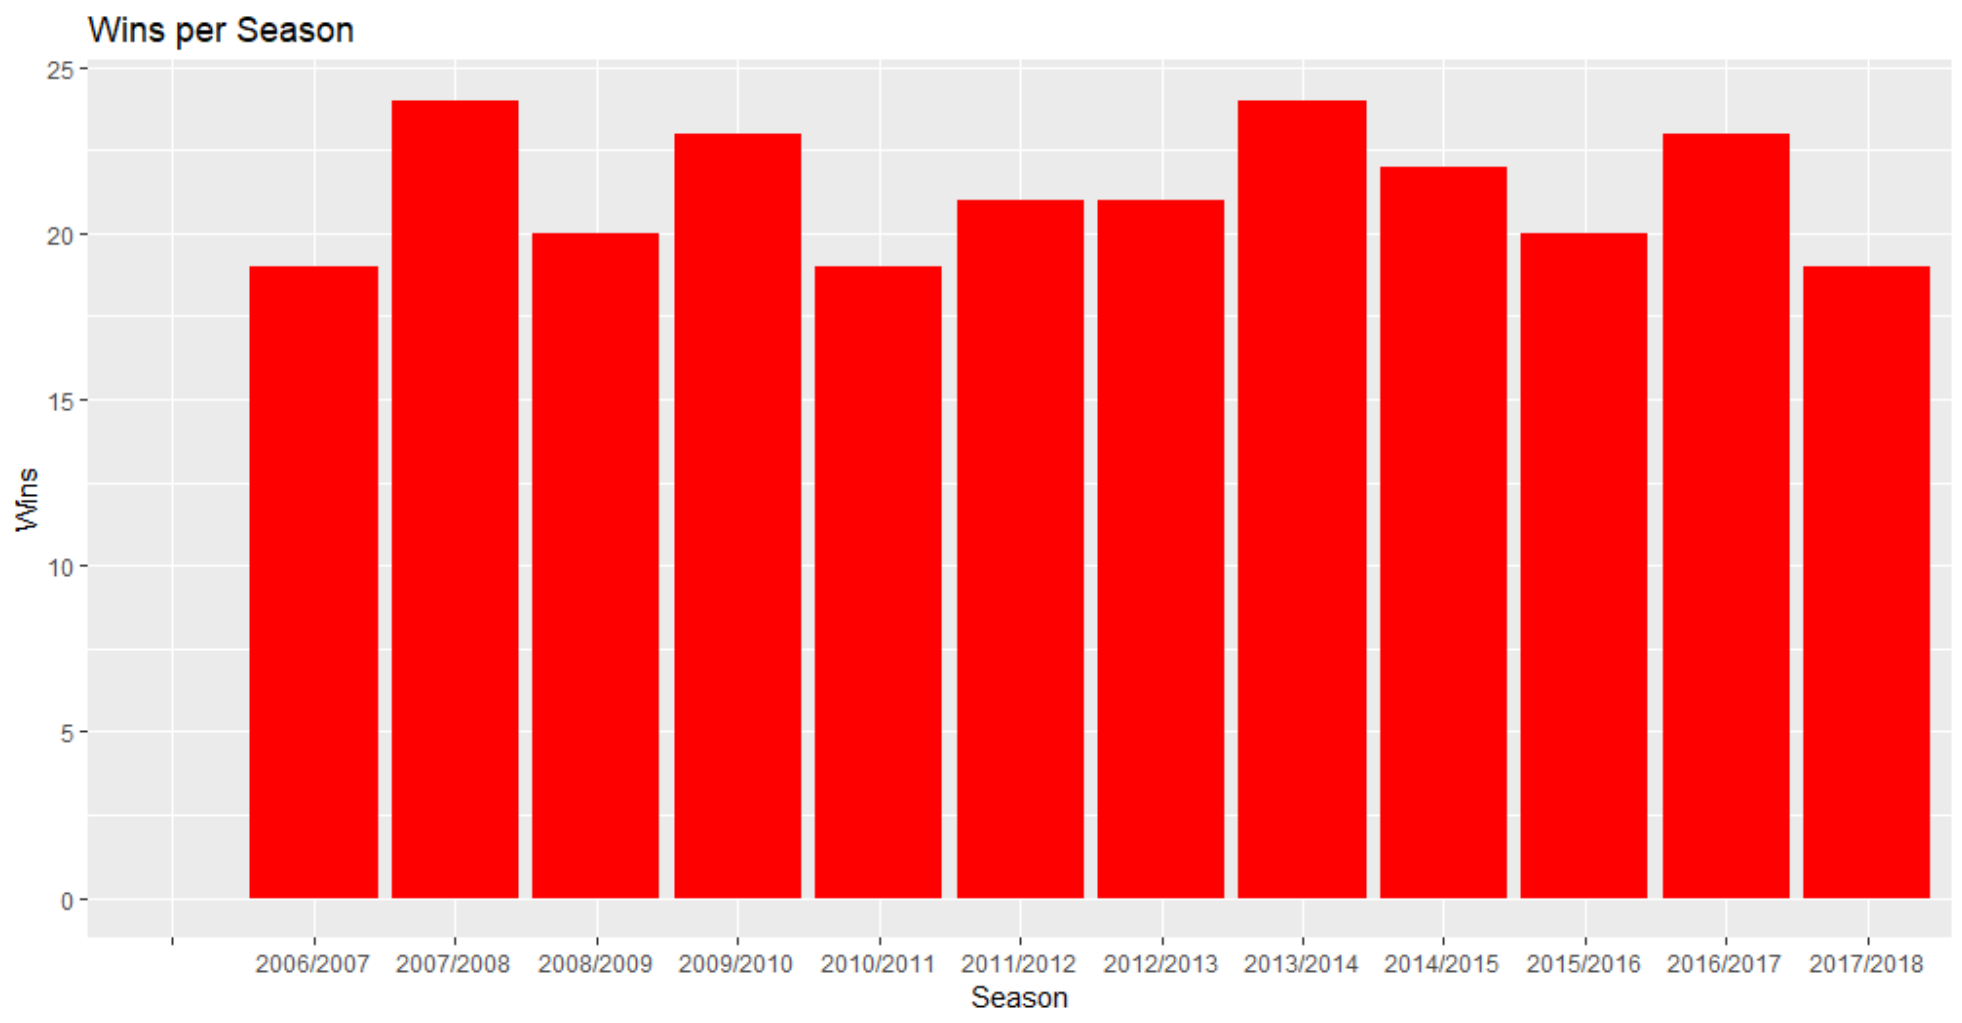
\includegraphics[width=\textwidth]{PS6b_Richardson}
This picture represents how many wins Arsenal had per season over the last 12 seasons. In the data, it can be seen what position of the league they were in in each season as well, which shows an interesting comparison. However, I was unaware of how to show the rank in the league above each season on this graphic.

\section{Shots per Season}
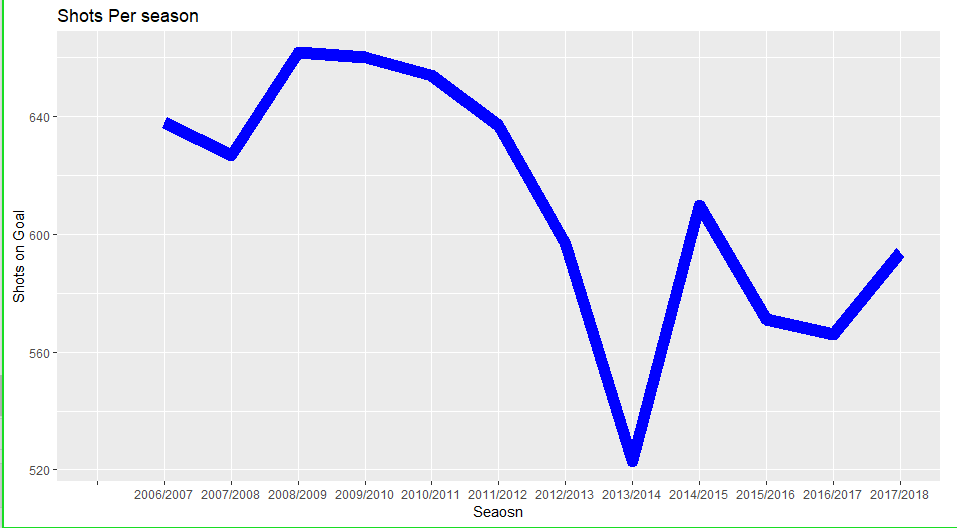
\includegraphics[width=\textwidth]{PS6c_Richardson}
This image shows how Arsenal's shot count has drastically changed over the last 12 seasons. Oddly enough, the shot count decreases most the year after Van Persie left for United.

\end{document}
